\section{Continuity} 

  \subsection{Sequences}

  \subsection{Continuous Functions}

    \begin{definition}[Continuous Function]
      A function $f$ between 2 topological spaces $(X, \mathscr{T}_{X})$ and $(Y, \mathscr{T}_{Y})$ is \textbf{continuous at $x \in X$} if the preimage of every open neighborhood of $f(x) \in Y$ is an open neighborhood of $x \in X$.
      \begin{equation}
        U_{f(x)} \in \mathscr{T}_{Y} \implies x \in f^{-1}(U_{f(x)}) \in \mathscr{T}_{X}
      \end{equation} 
      $f$ is said to be \textbf{continuous} (at all points) if the preimage of every open set in $Y$ is an open set in $X$.\footnote{Note that continuity of a function $f$ is not only determined by the function itself, but also by the topologies of $X$ and $Y$.}
    \end{definition}

    Note that to check if $f$ is continuous, it suffices to check that the preimage of every basis element of the topology of $Y$ under $f$ is open in $X$, since every open set in $Y$ can be constructed as the union of basis elements. More rigorously, an arbitrary open set $V$ of $Y$ can be written as 
    \begin{equation}
      V = \bigcup_{\alpha \in J} b_\alpha
    \end{equation}
    Then, 
    \begin{equation}
      f^{-1} (V) = f^{-1} \Big( \bigcup_{\alpha \in J} b_\alpha \Big) = \bigcup_{\alpha \in J} f^{-1} (b_\alpha)
    \end{equation}

    \begin{theorem}[Sufficient Properties for Continuity]
      Let $X, Y$, be topological spaces and let $f: X \longrightarrow Y$. Then, the following are equivalent. 
      \begin{enumerate}
        \item $f$ is continuous. 
        \item For every subset $A$ of $X$, $f(\bar{A}) \subset \bar{f(A)}$. 
        \item For every closed set $B$ in $Y$, the set $f^{-1} (B)$ is closed in $X$. 
      \end{enumerate}
    \end{theorem}  

    \begin{theorem}[Continuous Bijections]
      Suppose $f$ is bijective. Then 
      \begin{enumerate}
        \item $f$ is continuous implies for every open $U \subset Y$, $f^{-1} (U)$ is open in $X$. 
        \item $f^{-1}$ is continuous implies for every open $U \subset X$, $(f^{-1})^{-1} (U) = f(U)$ is open in $Y$.\footnote{Note by overloading the $-1$ exponent operator, the inverse and preimages are confusing. The inner represents the inverse and the outer represents the preimage. }
      \end{enumerate}
    \end{theorem} 

    \begin{theorem}[Analytic Continuity = Topological Continuity] 
      Given metric spaces with their induced metric topologies $(X, \mathscr{T}_X, d_X)$ and $(Y, \mathscr{T}_Y, d_Y)$. The following are equivalent. 
      \begin{enumerate}
        \item $f: X \rightarrow Y$ is continuous at $x$. 
        \item For every $\delta > 0$, there exists an $\epsilon = \epsilon(\delta) > 0$ such that for all $z \in X$, $d_X (x, z) < \epsilon \implies d_Y (f(x), f(x)) < \delta$.\footnote{This is the definition of continuity at a point in analysis.} 
      \end{enumerate}
    \end{theorem}
    \begin{proof}
      
    \end{proof}

  \subsection{Homeomorphisms}

    \begin{definition}[Homeomorphism]
      A bijective, bicontinuous function 
      \begin{equation}
        f: X \longrightarrow Y
      \end{equation}
      between two topological spaces is called a \textbf{homeomorphism} between $X$ and $Y$. If there exists at least one homeomorphism between $X$ and $Y$, then $X$ is said to be \textbf{homeomorphic} to $Y$. 

      \begin{figure}[H]
        \centering 
        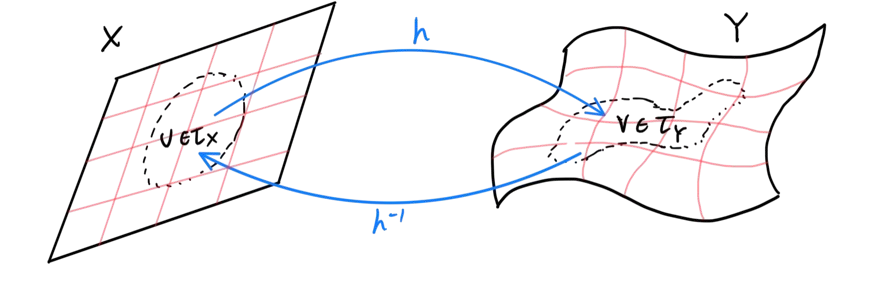
\includegraphics[scale=0.25]{img/Homeomorphism_of_Plane.PNG}
        \caption{The visual below shows a homeomorphism between the plane $X$ and the surface $Y$.}
        \label{fig:homeomorphism_plane}
      \end{figure}
    \end{definition}

    \begin{theorem}[Sufficient Properties of Homeomorphism]
      Suppose $f: X \rightarrow Y$ is a bijection. TFAE. 
      \begin{enumerate}
        \item $U \subset Y$ is open iff $f^{-1} (U)$ is open. 
        \item $U \subset X$ is open iff $f(U)$ is open. 
        \item $f$ is a homeomorphism. 
      \end{enumerate}
    \end{theorem} 

    \begin{example}[Comparability and Homeomorphic Spaces]
      Consider the set $X = \{a, b\}$ with the two topologies $\T_3 = \{\emptyset, \{a\}, X\}$ and $\T_4 = \{\emptyset, \{b\}, X\}$. They are not comparable but they seem ``similar'' in a way in that if we swap all the $a$'s and $b$'s in $\T_3$, then we get $\T_4$. We can make this rigorous by defining $f: (X, \T_3) \rightarrow (X, \T_4)$ with $f(a) = b, f(b) = a$, and showing that it is a homeomorphism. 
    \end{example}

    In fact, a homeomorphism $f$ is an equivalence relation between two topological spaces. This partitions the set of all topological spaces into \textbf{homeomorphism classes}. Analogous to how isomorphisms preserve algebraic structures, homeomorphisms preserve topological structure between topological spaces. 

    Additionally, not only does a homeomorphism give a bijective correspondence between points in $X$ and $Y$, but it also determines a bijection between \textbf{the set of all open sets in $X$ and $Y$} (that is, a bijection between their topologies)! This bijection then allows two spaces that are homeormophic to have the same topological properties. 

    \begin{proposition}
      A homeomorphism $f$ between two topological spaces $(X, \tau_{x})$ and $(Y, \tau_{Y})$ preserves all topological properties (e.g. separability, countability, compactness, (path) connectedness) of $X$ onto $Y$ and $Y$ onto $X$. 
    \end{proposition}

    \begin{definition}
      Suppose that $f: X \longrightarrow Y$ an injective continuous map with $X, Y$ topological spaces. Let $Z \equiv \im{f}$. Then, the function
      \begin{equation}
        f^\prime: X \longrightarrow Z \subset Y
      \end{equation}
      obtained by restricting the codomain of $f$ is bijective. If $f^\prime$ happens to be a homeomorphism of $X$ with $Z$, then we say that the map
      \begin{equation}
        f: X \longrightarrow Y
      \end{equation}
      is a \textbf{topological embedding}, or more simply an \textbf{embedding}, of $X$ in $Y$. 
    \end{definition}

    \begin{lemma}[Pasting Lemma, Gluing Lemma]
      Let $X = A \cup B$, where $A, B$ are closed in $X$. Let $f: A \longrightarrow Y$ and $g: B \longrightarrow Y$ be continuous. If 
      \begin{equation}
        f(x) = g(x) \text{ for all } x \in A \cap B
      \end{equation}
      Then $f$ and $g$ can be combined to form a continuous function $h: X \longrightarrow Y$, defined
      \begin{equation}
        h(x) \equiv \begin{cases}
          f(x) & x \in A \setminus B \\
          f(x) \text{ or } g(x) & x \in A \cap B \\
          g(x) & x \in B \setminus A
        \end{cases}
      \end{equation}
      This is shown in the following visual. 
      \begin{center}
          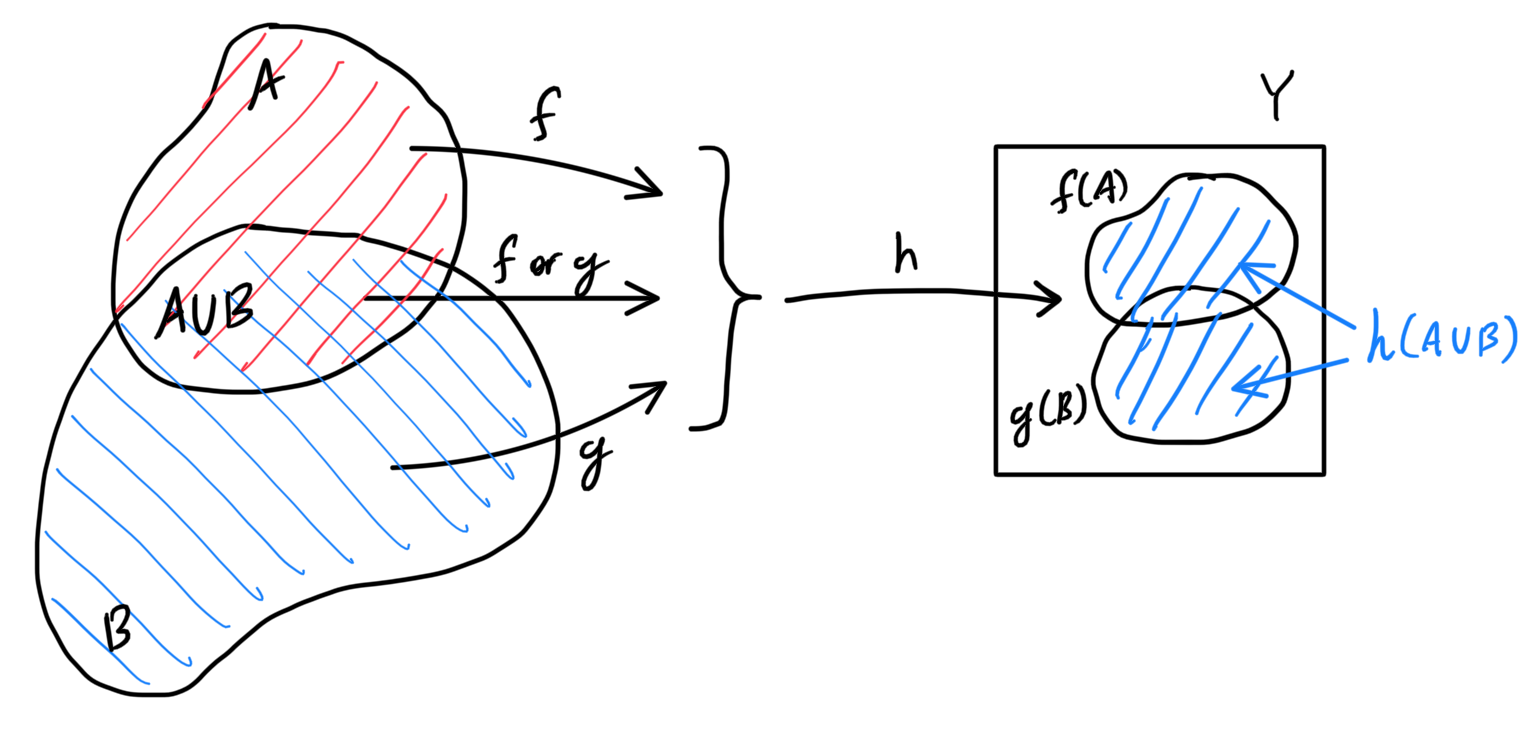
\includegraphics[scale=0.25]{img/Gluing_Lemma.PNG}
      \end{center}
    \end{lemma}

    \begin{theorem}
      Let $f: A \longrightarrow X \times Y$ be given by the equation 
      \begin{equation}
        f(a) \equiv \big( f_1 (a), f_2(a) \big)
      \end{equation}
      Then $f$ is continuous if and only if the function $f_1: A \longrightarrow X$ and $f_2: A \longrightarrow Y$ are continuous. 
    \end{theorem}

    However, there is no useful criterion for the continuity of a mapping 
    \begin{equation}
      f: X \times Y \longrightarrow A
    \end{equation}
    if the domain of $f$ is a product space. One might conjecture that this $f$ is continuous if it is continuous in each variable separately, but this is in fact not true. 

